\documentclass[14pt]{extarticle}

\usepackage[T2A]{fontenc}               % fonts
\usepackage[utf8x]{inputenc}             % UTF-8
\usepackage[english,russian]{babel}     % russian
\usepackage{cmap}                       % russian search in pdf
\usepackage[14pt]{extsizes}             % for compatibility

\usepackage{indentfirst}        % first string indention

\usepackage{graphicx}           % graphics
\usepackage{ltxtable}           % tables

\usepackage{amsmath}            % math
\usepackage{amsfonts}           % math fonts
\usepackage{amssymb}            % math symb
\usepackage[a4paper, left=3cm, right=2cm, top=2cm, bottom=3cm]{geometry}   % pagesize

\usepackage{color}
\usepackage[table]{xcolor}
\definecolor{light-gray}{gray}{0.9}

\usepackage{soul}               % \so{} & \ul{} - source and underline
\usepackage{soulutf8}           % UTF-8 for soul
\usepackage{verbatim}           % \verb{} and verbatim environment
\usepackage{listings}           % source code `bl
\lstset{
        escapeinside={\#@}{@},
        extendedchars=\true,
        numbers=left,
        inputencoding=utf8,
        keepspaces=true,
        basicstyle=\footnotesize\ttfamily,
        backgroundcolor=\color{light-gray},
        tabsize=3
}

\usepackage{fancyhdr}
\pagestyle{fancy}
\fancyhf{}                              % clear header and footer
\fancyfoot[C]{\thepage}                 % page number
\renewcommand{\headrulewidth}{0.0pt}
\renewcommand{\footrulewidth}{0.0pt}
%\fancyhead[HR]{\slshape \leftmark}
%\fancyhead[HL]{\footnotesize{\scshape \leftmark}}
%\fancyhead[HR]{\footnotesize{\scshape\nouppercase{\rightmark}}}



\linespread{1.4}                % line interval ~1.5
\renewcommand{\rmdefault}{ftm}

%% SPECIFIC PART
\usepackage[raggedright,sf]{titlesec}
\usepackage{lipsum}
\usepackage{multirow}
\usepackage{tabularx}
\usepackage{placeins}
\usepackage{totcount}
\usepackage{float}
\usepackage[hidelinks]{hyperref}
\usepackage[numbers,sort&compress]{natbib}
\usepackage{caption}
\usepackage{subcaption}
\frenchspacing
\setcounter{page}{1} %TODO fix
\bibliographystyle{utf8gost705u}
\makeatletter % [1] -> 1.
\renewcommand\@biblabel[1]{#1.}
\makeatother
\addto\captionsrussian{\def\refname{}}
\regtotcounter{page}
\regtotcounter{figure}
\regtotcounter{table}
\captionsetup{justification=centering,labelsep=period}
%\captionsetup[table]{aboveskip=0pt,belowskip=0pt}
%% END OF SPECIFIC PART


\usepackage{tocloft}
\renewcommand{\cftsecleader}{\cftdotfill{\cftdotsep}}

\newcommand{\myparagraph}[1]{\paragraph{#1}\mbox{}\\}

\begin{document}

	\tableofcontents
	\clearpage

	\section{Введение}
	\paragraph{}
Среди специалистов в области психолингвистики, когнитивной психологии и философии познания существует гипотеза о существовании  «языка мысли» или семантического языка. Этот язык является представлением мысли, а перевод с естественного языка на семантический является процессом понимания. Семантический язык универсален и присущ всем людям с момента рождения. В своей книге «Язык мысли» («The Language of Thought»\cite{fodor}) Джерри Фодор называет этот язык «Ментализом». Неотъемлемой частью процесса восприятия естественного языка является распознавание слов. Человек способен распознать слова в написанном тексте, даже при отсутствии разделительных символов и наличии орфографических ошибок. Специалисты в области когнитивной психологии достаточно давно изучают психологические аспекты распознавания слов в тексте и формулируют различные модели этого процесса: распознавание по форме, последовательное и параллельное буквенное распознавание\cite{larson}. 
\paragraph{}
Одной из задач области обработки текста на естественном языке является получение некоторого машинного представления смысла обрабатываемого текста. Решение данной задачи включает в себя несколько фаз обработки текста, на первой из которых необходимо произвести распознавание слов.

\newpage
\subsection{Описание предметной области}
Обработка текста на естественнном языке или компьютерная лингвистика - междисциплинарное научное направление, объединяющее знания и методы лингвистики и области искусственного интеллекта. Объектом исследования компьютерной лингвистики является текст на естественном языке. Текст можно рассматривать как выражение смысла или мысли. Следует отметить, что для одной и той же мысли может существовать несколько формулировок на естественном языке. Этот факт является аргументом в пользу справедливости гипотезы о существовании “языка мысли”. Постижение смысла, содержащегося в обрабатываемом тектсе, и формирование его некоторого формального машинного представления и есть одна из основных задач компьютерной лингвистики. Возможность получения формального представления смысла является необходимой предпосылкой для создания ителлектуальных информационных систем. В рамках компьютерной лигвистики существуют различные математические модели, используемые для описания естественного языка. В современной компьютерной лингвистике большое применение имеют вероятностные модели языка.

\paragraph{}
В рамках автоматической обработки текста выделяют следующие фазы:
\begin{itemize}
\item
графематический анализ;
\item
морфологический анализ;
\item
синтаксический анализ;
\item
семантический анализ.
\end{itemize}


\subsection{Цель работы}
Разработать подход предсентактического аннотирования текста, позволяющий выполнять раземтку текста. Разработанный подход должен позволять выполнять аннотирование текста, содержащего дефекты. На основе найденного подхода необходимо реализовать программный модуль предсинтаксического аннотирования текста. Программный модуль должен интегрироваться в разрабатываемую систему семантического анализа. Подход должен позволять адаптировать программный модуль для выполнения аннотирования текстов на разных алфавитных языках.

\subsection{Актуальность решаемой задачи}
Поставленная задача актуальна ввиду специфичных требований к модулю предсинтаксического аннотирования текста, связанных с подходом разрабатываемым в рамках системы семантического анализа. 
К специфичным требованиям относятся следующие требования
устойчивость к дефектам 
возможность адаптирования для работы с новыми алфавитными языками
результат работы модуля должен ссылаться на словарные статьи графового словаря, используемого в системе семантического анализа
Устойчивость к дефектам позволит системе семантического анализа обрабатывать тексты, не проходящие предварительную орфографическую проверку. Такие текты наиболее широко распространены в различных веб-ресурсах, веб-форумах, где пользователи набирают текс в спешке и не уделяют должного внимания проверке своих текстов. Анализ таких текстов представляет широкий интерес для различных информационных систем и может быть использован, например,  для исследования паттернов поведения пользователей. Другим примером текстов, содержащих дефекты является тексты, полученные в результате оптического сканирования. К данному классу текстов относятся тексты, существующие на бумажном носителе и не доступные в электронном виде, например, архивные документы. Анализ таких текстов так же представляет штрокий интерес для информационных систем, используемых в некоторых сферах.
	\FloatBarrier
	\clearpage

	\section{Существующие подходы}
	На сегодняшний день существует большое количество фреймворков, предназначенных для построения систем автоматической обработки текста на естественном языке. В состав некоторых фреймворков входят модули графематического анализа. Существуют различные методы, применяемые при выполнении графематического анализа: использование правил, словарный поиск, машинное обучение, эвристика.
\begin{table}[H] \small
	\centering
	\label{t:thyp_gd1}
	\begin{tabular}{ | c | c | c | c |}
		\hline
		Название 							& Метод 				& Языки 		& Платформа 				\\ \hline
		АОТ\cite{web.aot}					& словарный поиск		& русский,		& GNU/Linux,			\\
											&						& английский	& Microsoft Windows(C++)\\ \hline
		Stanford CoreNLP\cite{web.corenlp}	& эвристика				& английский	& JVM (Java)			\\ \hline
		Apache OpenNLP\cite{web.opennlp}	& использование правил,	& английский	& JVM (Java)			\\
											& машинное обучение		& 				&						\\ \hline
		FreeLing\cite{web.freeling}			& использование правил	& русский,		& GNU/Linux (C++)		\\
											&						& английский,	&						\\
											&						& и др.			&						\\ \hline
		Solarix\cite{web.solarix}			& использование правил	& русский,		& GNU/Linux,			\\ 
											&						& английский	& Microsoft Windows(C++)\\
		\hline
	\end{tabular}
	\caption{Проекты, включающие модули графематического анализа}
\end{table}
Использование правил заключается в использовании правил, задающих границы словоформ. Модули, основанные на использовании правил, обычно требуют для своей работы библиотеку правил. Такие библиотеки могут составляться отдельно для разных языков. Обычно, правила представляют собой регулярные выражения, задающие границы словоформ. Словарный поиск заключается в поиске словоформ в морфологическом словаре. Машинное обучение широко применяется в системах семантического анализа как на этапе разметки текста, так и на последующих фазах. Использование данного подхода сопряжено с составлением обучающего множества. Обычно выполняется совмещение нескольких подходов, для чего используются некоторые эвристические правила.

\subsection{Необходимость нового подхода}
Среди существующих решений нет решений, удовлетворяющих одновременно всем поставленным требованиям.
Существующие модули, выполняющие графематический анализ, разрабатываются в составе фреймворков, включающих модули, выполняющие другие фазы автоматической обработки текста. В связи с этим, на данные модули наложены некоторые ограничения, обусловленные глобальным подходом к обработке текста на естественном языке, применяемом в том или ином фреймворке. В разрабатываемой системе семантического анализа используется подход к анализу естественного языка, лишь частично согласующийся с существующими подходами. Ввиду этого, разрабатываемый модуль предсинтаксического аннотирования текста должен решать дополнительные задачи, непредусмотренные в существующих модулях. Примером такой задачи можно назвать связывание найденных токенов с узлами графового словаря, содержащего узлы разных типов и позволяющий производить связывание словоформ со смысловыми узлами. Так же следует отметить, что существующие модули графематического анализа работают лишь с некоторыми языками, вследствие чего может понадобиться реализация модуля определения языка, что усложняет архитектуру системы. Ввиду сказанного необходимо разработать новый подход и основанный на нем программный модуль.
	\FloatBarrier
	\clearpage

	\section{Разработанный подход}
	В данной работе предлагается новый подход к предсинтаксическому аннотированию текста на естественном языке. Данный подход отличается от существующих тем, что: 
\begin{itemize}
\item
позволяет аннотировать текст, содержащий дефекты;
\item
универсален для разных языков;
\item
допускает неоднозначность результата аннотирования.
\end{itemize}
В случае разметки текста по правилам такие дефекты, как пропущенные или, наоборот, лишние разделительные символы, не могут быть учтены. Причиной этого является то, что алгоритмы разметки текста, использующие регулярные выражения, ориентируются на непосредственное присутствие того или иного символа или символа, принадлежащего какому-либо типу. Универсальность разработанного подхода выражается в том, что модуль, разработанный на основе данного подхода может быть адаптирован для работы с несколькими языками без изменения кода самого модуля. Адаптация заключается в обучении модуля на той или иной тренировочной выборке и в предоставлении необходимых ресурсов: морфологического словаря и частотных списков n-грамм.
Предлагаемый подход состоит из двух фаз:
\begin{itemize}
\item
фаза разметки текста;
\item
фаза словарного поиска.
\end{itemize}
Для предварительной разметки текста введена фаза разметки текста. По-другому задача разметки текста называется графематическим анализом. Предварительная разметка текста представляет собой поиск границ токенов. Другими словами, задача, выполняемая на фазе разметки текста состоит в преобразовании последовательности символов, представляющей текст на естественном языке, в последовательность найденных токенов. Токенами могут быть словоформы и цифровые комплексы. Следует подчеркнуть, что результат работы фазы разметки текста однозначен, то есть для данной последовательности символов текста может быть получена одна и только одна последовательность токенов. 
\begin{figure}[H]
	\centering
	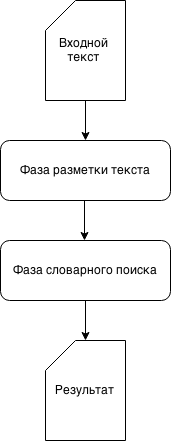
\includegraphics[scale=0.7]{img/approach.png}
	\caption{Фазы разработанного подхода}
\end{figure}
Впоследствии результат, полученный на фазе разметки текста, передается на вход фазе словарного поиска. Эта фаза введена для достижения учета возможности наличия в тексте дефектов; основная ее задача - установить корректность найденных словоформ путем их поиска в словаре и, в случае неудачного поиска, найти возможные варианты корректировки.

\subsection{Фаза разметки текста}
Фаза разметки текста выполняет предварительную разметку текста. Для достижения возможности адаптации разработанного программного модуля для работы с разными языками на данной фазе принято решение использовать алгоритм, относящийся к классу алгоритмов машинного обучения. Была проанализирована сущность процесса разделения последовательности символов на отдельные единицы - токены. С одной стороны, данный процесс может быть представлен конечным автоматом и описан некоторой формальной грамматикой. Такой взгляд на данный процесс носит детерминированный характер и требует четкого задания формальной грамматики, что может представлять дополнительную трудоемкость при адаптации модуля для работы с текстами на разных языках. С другой стороны, процесс разделения последовательности символов на отдельные единицы может быть рассмотрен как стохастический, причем двойственный. Во-первых, мы имеем непрерывную последовательность символов. А во-вторых, данная последовательность представляет собой последовательность токенов. Связь этих двух последовательностей можно рассмотреть с вероятностной точки зрения. Данный взгляд на процесс разделения последовательности символов хорошо отображается семантикой скрытой марковской модели. Исходя из этого, было принято решение использовать скрытую марковскую модель (СММ). 

Использование СММ предполагает подбор параметров модели, правдоподобно описывающих процесс. Подбор параметров представляет собой обучение модели. В данной работе используется алгоритм обучения с учителем. Для работы алгоритма обучения с учителем необходимо предоставить обучающее множество. Формирование обучающего множества является частью работы и выполняется на основе использования размеченного лингвистического корпуса. Обученная скрытая марковская модель используется для анализа входного текста и выполнения предварительной разметки текста.

\begin{figure}[H]
	\centering
	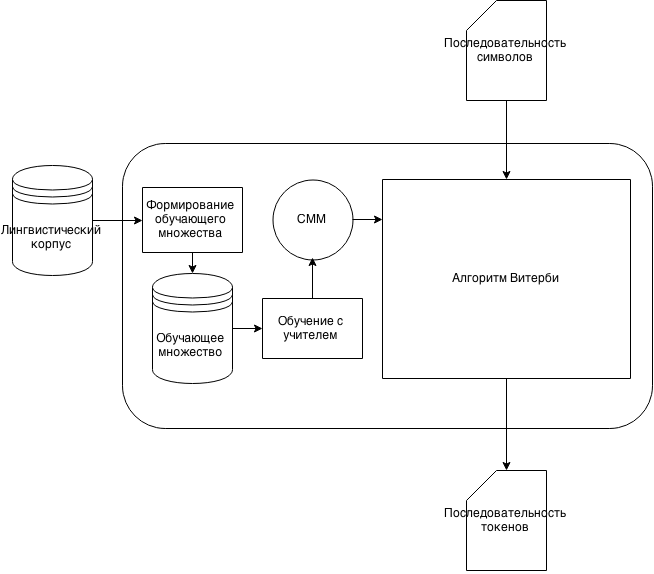
\includegraphics[scale=0.7]{img/tokenization.png}
	\caption{Фаза разметки текста}
\end{figure}

\subsubsection{Скрытая марковская модель}
Скрытая марковская модель - статистическая модель, широко применяемая в задачах распознавания речи, биоинформатики, сжатия данных, а также в области искусственного интеллекта. Процессы, протекающие в реальном мире проявляются в виде сигналов, воспринимаемых наблюдателем. Нередко источник сигналов непостижим наблюдателем в явном виде. Наблюдатель может судить о состоянии источника сигнала лишь по полученным сигналам, которые могут быть подвержены влиянию шумов, вследствие чего задача определения состояния источника сигналов становится нетривиальной. СММ является вероятностной моделью, широко применяемой в задачах определения внутреннего состояния процессу по его внешним проявлениям. СММ представляет собой обучаемый стохастический конечный автомат и может быть рассмотрена как специфическая форма динамической байесовской сети.

Впервые скрытые марковские модели начали применяться в области распознавания речи. Историю СММ можно разделить на две части \cite{kouemou}. С одной стороны это история Марковского процесса и Марковских цепей, а с другой - история алгоритмов, разрабатывавшихся для решений различных задач с помощью СММ. Андрей Андреевич Марков описал Марковские цепи в 1906 г., когда получил первые теоретические результаты исследования стохастических процессов. Марковский процесс может быть рассмотрен как процесс изменения некоторой случайной величины, который удовлетворяет Марковскому свойству. Марковское свойство заключается в том, что условное распределение вероятностей будущих состояний зависит от состояния, в котором процесс находится на данный момент, и не зависит от предыстории состояний. Другими словами, будущее не зависит от прошлого и зависит только от настоящего. В 1940-е годы с бурным развитием компьютерных наук многие ученые из разных областей начали искать применение как детерминированных, так и стохастических автоматов для решения своих задач. В 1977 году были обобщены накопившиеся знания и опыт использования EM-алгоритма \cite{dempster1977maximum}. 

EM-алгоритм является классическим алгоритмом, используемым в математической статистике для нахождения максимально правдоподобной оценки неизвестных параметров вероятностных моделей. EM-алгоритм представляет собой итеративный алгоритм. Каждая итерация алгоритма состоит из двух шагов. На E-шаге (expectation) вычисляется ожидаемое значение функции правдоподобия, при этом скрытые переменные рассматриваются как наблюдаемые. На M-шаге (maximization) вычисляется оценка максимального правдоподобия, таким образом увеличивается ожидаемое правдоподобие, вычисляемое на E-шаге. Затем это значение используется для E-шага на следующей итерации. Алгоритм выполняется до сходимости. Алгоритм Баума-Велша является частным случаем EM-алгоритма и применяется для нахождения неизвестных параметров скрытой марковской модели. Алгоритм Витерби был предложен Эндрю Витерби в 1967 году для декодирования сверточных кодов \cite{viterbi1967error}. Этот алгоритм относится к классу алгоритмов динамического программирования и позволяет найти наиболее правдоподобную последовательность скрытых состояний процесса, называемую путем Витерби.

Скрытая марковская модель представляет собой обучаемый стохастический конечный автомат. Выделяют два вида СММ: для дискретных наблюдений (событий) и непрерывных сигналов. В работе рассмотрена дискретная СММ ввиду дискретного характера данных, что будет обосновано далее. Скрытая марковская модель объединяет в себе два стохастических процесса.
\begin{itemize}
\item
Первый процесс представляет собой переходы между состояниями, скрытыми от наблюдателя.
\item
Второй процесс представляет собой появление некоторых событий, которые известны наблюдателю. Распределения вероятностей появления этих событий зависят от скрытого состояния, в котором находится система.
\end{itemize}


Для формального описания модели используются следующие математические объекты:
\begin{itemize}
	\item
	Количество скрытых состояний модели \(N\). Несмотря на то, что информация о том, в каком состоянии модель находится в конкретный момент времени, не доступна для наблюдателя, множество всевозможных состояний наблюдателю известно:
	\begin{align} 
		S = \{ S_1, S_2, ..., S_N \};
	\end{align}
	\item
	Количество различных символов наблюдений \(M\). Символы наблюдений соответствуют регистрируемым событиям, порождаемым наблюдаемым процессом. Множество различных символов наблюдений называется алфавитом наблюдений
	\begin{align} 
		V = \{ v_1, v_2, ..., v_M \};
	\end{align}
	\item
	Матрица вероятностей переходов между скрытыми состояниями
	\begin{align} 
		&A = \{ a_{ij} \}, \\
		&a_{ij} = P[q_{t + 1} = S_j | q_t = S_i];
	\end{align}
	\item
	Распределение вероятностей появления символов в j-ом состоянии
	\begin{align}
		&B = \{ b_j(k) \}; \\ 
		&b_j(k) = P(v_k | t = k, q_t = S_j);
	\end{align}
	\item
	Распределение вероятностей начального состояния
	\begin{align}
		&\pi = \{\pi_i\}; \\
		&\pi_i = P(q_1 = S_i). 
	\end{align}
\end{itemize}

Таким образом, чтобы полностью задать СММ, необходимо определить параметры модели (\(N, M\)), определить алфавит символов наблюдений и вероятностные характеристики модели \(A, B\) и \(\pi\). Для компактной записи полного задания параметров модели используется нотация
\begin{align}
	\lambda = (A, B, \pi).
\end{align}

Определены три типовые задачи, решаемые при использовании СММ в различных прикладных задачах \cite{Rabiner89atutorial}:
\begin{itemize}
	\item
	Вычисление \(P(O|\lambda)\), вероятности проявления последовательности событий, при данных последовательности событий \(O=O_1O_2...O_T\) и модели \(\lambda = (A, B, \pi)\);
	\item
	Выбор последовательности скрытых состояний \(Q=q_1q_2...q_T\), которая наилучшим образом объясняет последовательность наблюдений, при данных последовательности событий \(O=O_1O_2...O_T\) и модели \(\lambda = (A, B, \pi)\);
	\item
	Подбор параметров модели \(\lambda = (A, B, \pi)\) для максимизации \(P(O|\lambda)\).
\end{itemize} 

Другими словами, первую задачу можно определить как определение вероятности того, что полученная последовательность наблюдений порождена данной моделью. С другой стороны, решение данной задачи может потребоваться для оценки правдоподобия подобранных параметров модели, что может потребоваться при решении задачи подбора параметров модели или выбора конкретной модели из нескольких. Первая задача решается с помощью алгоритма ``прямого-обратного'' хода. Данный алгоритм имеет вычислительную сложность \(O(T * N^T)\), где \(T\) - длина последовательности, \(N\) - число скрытых состояний модели. Решение второй задачи представляет собой постижение скрытого процесса. Другими словами, решение данной задачи позволяет найти наиболее вероятную последовательность скрытых состояний системы по имеющейся последовательности наблюдений. Последовательность скрытых состояний модели называется путем Витерби, для нахождения которого используется алгоритм Витерби, имеющий вычислительную сложность \(O(T * |S|^2)\), где \(|S| = N\) - количество скрытых состояний модели, а \(T\) - размер входной последовательности наблюдений. Здесь следует отметить, что, применительно к конкретной задаче, количество скрытых состояний может быть определено, т.е. быть величиной постоянной, а значит, согласно правилам асимптотической оценки \cite{clrs} сложности алгоритмов, сложность алгоритма Витерби линейна относительно размера входной последовательности. Третья задача является задачей оптимизации параметров модели с целью наилучшего объяснения наблюдаемых последовательностей событий. По-другому данная задача называется задачей обучения, причем данный вид обучения является обучением без учителя и решается с помощью алгоритма Баума-Велша.

Приведем пример системы, описываемой скрытой марковской моделью. Пусть в комнате находятся два человека. У первого человека завязаны глаза, перед вторым человеком стоят \(N\) урн, наполненных шарами разного цвета. Второй человек начинает брать шары из разных урн в произвольном порядке и называть цвета взятых шаров. При этом он не говорит, из какой именно урны он взял тот или иной шар. 
\begin{figure}[H]
	\centering
	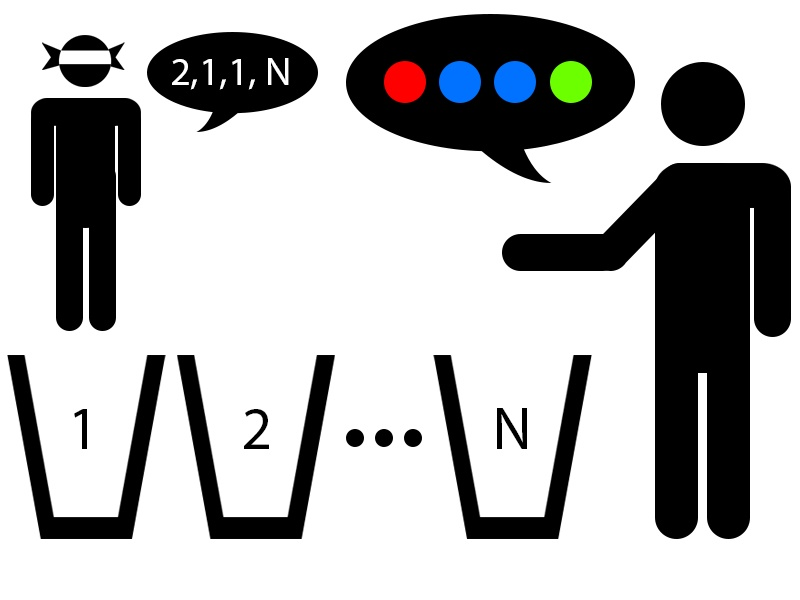
\includegraphics[scale=0.7]{img/hmm.jpg}
	\caption{Иллюстрация процесса, описываемого СММ}
\end{figure}
Используя СММ для описания этого процесса, первый человек может пытаться угадывать, из какой урны какой шар был взят. Наблюдаемым процессом в данном случае является речь человека, называющего цвета взятых шаров, а скрытым процессом является выбор им той или иной урны. В этой ситуации элементами множества наблюдений являются цвета шаров, а элементами множества скрытых состояний являются номера урн.

\subsubsection{Использование скрытой марковской модели для разметки текста}
Текст на естественном языке также можно рассматривать как два стохастических процесса, описываемых скрытой марковской моделью. В таком случае наблюдаемым процессом можно считать последовательность символов текста, а скрытым процессом - принадлежность того или иного символа словоформе, ее границе или непринадлежность символа словоформе. Возможно введение дополнительных скрытых состояний для описания различных типов словоформ. Множество наблюдений представляет собой типы символов, из которых состоит текст. В простейшем случае множество наблюдений может представлять собой подмножество кодов символов некоторого набора символов, например, Юникода.
\begin{itemize}
	\item
	Определим множество скрытых состояний:
	\begin{align}
		&S = \{ S_{in}, S_{out}, S_{bnd}\}, \text{где}\\
		&S_{in} - \parbox[t]{20em}{состояние, соответствующее расположению символа внутри словоформы,} \nonumber \\
		&S_{out} - \parbox[t]{20em}{состояние, соответствующее расположению символа вне словоформы,} \nonumber \\
		&S_{bnd} - \parbox[t]{20em}{состояние, соответствующее расположению символа на границе словоформы.} \nonumber
	\end{align}

	\item
	Определим множество наблюдений:
	\begin{align}
		&V = \{ v | v \in C\}, \text{где} \\
		&C - \parbox[t]{25em}{некоторое подмножество символов Юникода} \nonumber
	\end{align}
\end{itemize}

Для полного определения скрытой марковской модели, которую можно использовать для разметки текста, необходимо также задать матрицу вероятностей переходов между скрытыми состояниями \(A\), вектор распределений вероятностей появления символов \(B\) и распределение вероятностей начального состояния \(\pi\). Для подбора данных параметров модели необходимо применение какого-либо метода обучения. В работе применяется метод обучения с учителем, который рассмотрен в следующем разделе.

\subsubsection{Обучение скрытой марковской модели с учителем}
Как было упомянуто выше, алгоритм Баума-Велша является обучением без учителя. В данном алгоритме производится подбор параметров модели для достижения наиболее правдоподобного соответствия последовательности скрытых состояний \(Q=q_1q_2...q_T\) последовательности наблюдений \(O=O_1O_2...O_T\). При отсутствии каких-либо начальных сведений о вероятностях переходов между состояниями или распределениях вероятностей появлений символов для различных скрытых состояний, данный алгоритм позволит обучить модель для распознавания моментов смены скрытых состояний, однако сами состояния не будут привязаны к конкретному типу.

В данной работе используется метод обучения скрытой марковской модели с учителем. Метод основан на частотном определении вероятности. Для обучения используется обучающая выборка или обучающее множество, представляющее собой множество пар последовательностей наблюдений и соответствующих им последовательностей скрытых состояний. Принимая на вход обучающую выборку, алгоритм обучения производит подбор параметров модели. Опишем работу алгоритма. Пусть дано обучающее множество
\begin{align}
T = \{(O_i, Q_i) | 0 \le i \le N\} \text{,}
\end{align}
где \(N\) - количество элементов обучающего множества. Для \(z\) от \(0\) до \(N\) необходимо
\begin{itemize}
\item
инкрементировать \(\pi_i\), где \(O_{z0}\) = \(S_i\);
\item
прибавить к \(a_{ij}\) число, равное количеству переходов из состояния \(S_i\) в \(S_j\) в данной последовательности;
\item
прибавить к \(b_j(k)\) количество появлений символа \(V_k\) в состоянии \(S_j\).
\end{itemize}
Так как может оказаться, что некоторые элементы \(\pi_i = 0\), \(a_{ij} = 0\) или \(b_j(k) = 0\), то необходимо произвести корректировку, которая заключается в прибавлении \(1\) ко всем элементам.
Теперь можно вычислить окончательные параметры модели следующим образом:
\begin{align}
	\pi_i &\leftarrow \frac{\pi_i}{\displaystyle\sum_{k} \pi_k}; \\
	a_{ij} &\leftarrow \frac{a_{ij}}{\displaystyle\sum_{k} a_{ik}}; \\
	b_j(k) &\leftarrow \frac{b_j(k)}{\displaystyle\sum_{t} b_j(t)}.
\end{align}

\subsubsection{Формирования обучающего множества}
В предыдущем разделе был рассмотрен алгоритм обучения скрытой марковской модели с учителем, который применяется в данной работе. Данный алгоритм принимает на вход тренировочное множество, на основе которого выполняется обучение модели. Исходя из этого, необходимо решить задачу о составлении тренировочного множества.


\subsection{Фаза словарного поиска}
Фаза словарного поиска принимает на вход результат разметки текста, полученный на фазе разметки текста. Как было сказано выше, результатом работы первой фазы является список найденных токенов. Задача фазы словарного поиска проверить корректность найденных токенов и, возможно, произвести коррекцию результата. Результат может быть неоднозначным. Т.е. возможно существование нескольких вариантов разбиения исходной последовательности символов на токены, в таком случае список результатов ранжируется в соответствии с некоторым критерием, о котором будет сказано ниже. Поиск и проверка корректности словоформ осуществляется словарным поиском по графовому словарю, о котором будет рассказано ниже. Результат разбиения представляется линейно упорядоченным множеством \cite{vereshagin_shen} ссылок на узлы словоформ графового словаря, о котором будет сказано ниже. 

Сначала производится прямой поиск по словарю. Если в результате прямого поиска словоформа в словаре не найдена, то выполняется нечеткий поиск. В ходе нечеткого поиска производятся попытки найти словоформы, полученные объединением словоформ, расположенных последовательно. Также могут производиться попытки найти отдельные словоформы, составляющие один токен, найденный на первой фазе. Метрикой, используемой алгоритмом нечеткого поиска является редакционное расстояние.

Как было сказано, в результате нечеткого поиска может быть получено несколько вариантов разметки текста. В таком случае производится ранжирование списка результатов, которое учитывается на последующих фазах автоматической обработки текста, принимающих на вход результат предсинтаксического аннотирования текста. Ранжирование производится на основе критерия, учитывающего вычисленное редакционное расстояние и вероятностный критерий, определенный в рамках модели n-грамм \cite{probling}.

\begin{figure}[H]
	\centering
	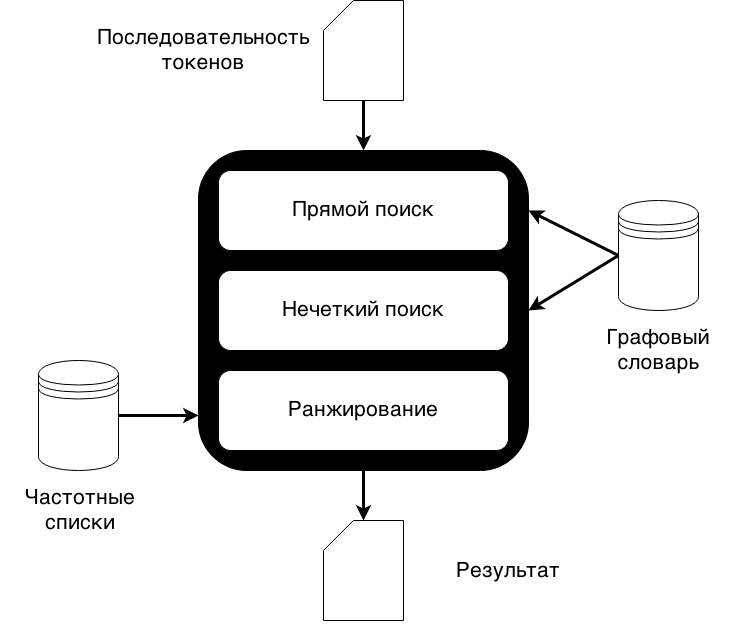
\includegraphics[scale=0.5]{img/dictphase.png}
	\caption{Фаза словарного поиска}
\end{figure}

\subsubsection{Графовый словарь}
Разработанный в данной работе подход применяется в программном модуле, входящем в состав системы семантического анализа. Данная система семантического анализа основана на такой лингвистической концепции, как фреймовая семантика \cite{fillmore1976frame}. Используемые алгоритмы анализа текста работают с внутренним словарем, имеющим графовую структуру. Данный словарь объединяет в себе морфологический словарь и семантическую сеть. В рамках графовой структуры словаря определены узлы трех типов:
\begin{itemize}
	\item
	семантические узлы;
	\item
	узлы лексем;
	\item
	узлы словоформ.
\end{itemize}
Узлы графового словаря связаны ребрами следующих типов:
\begin{itemize}
	\item
	ребра, соответствующие семантическим отношениям;
	\item
	ребра, связывающие семантические узлы с узлами лексем и выражающие возможность представления того или иного понятия конкретной лексемой в тексте;
	\item
	ребра, связывающие лексемы с их словоформами.
\end{itemize}
Семантический узел представляет собой синонимический ряд (``синсет'' \cite{wordnet}). Семантические узлы могут быть связаны ребрами, выражающими такие семантические отношения, как:
\begin{itemize}
\item
гиперонимия;
\item
гипонимия;
\item
``часть -- целое'';
\item
меронимия;
\item
антонимия;
\item
и др.
\end{itemize}
Результатом работы модуля аннотирования является список найденных токенов, представляющий собой ссылки на найденные словоформы.
\begin{figure}[H]
	\centering
	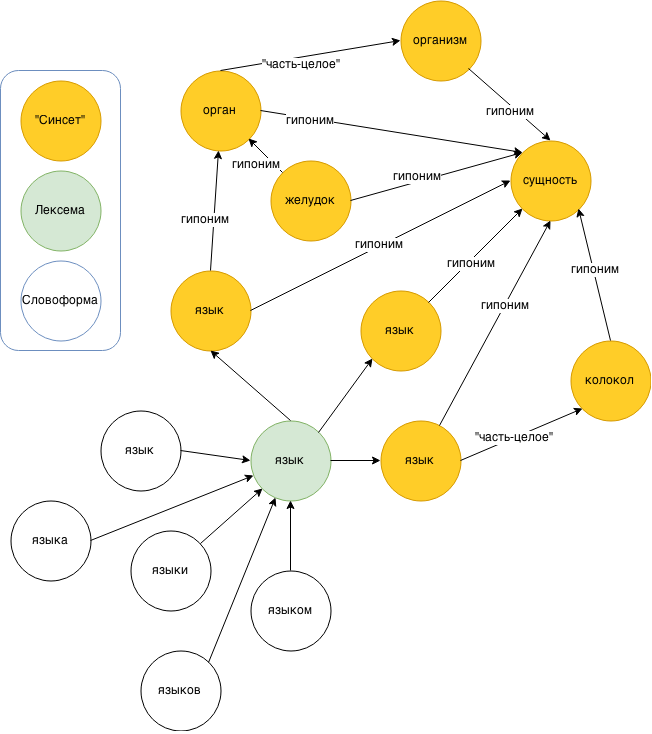
\includegraphics[scale=0.5]{img/dict.png}
	\caption{Пример фрагмента графового словаря}
\end{figure}

\subsubsection{Дерево поиска}
Алгоритмы, используемые на данной фазе, работают с графовым словарем. Для избежания полного сканирования узлов словоформ во время операций прямого и нечеткого поиска по словарю используется префиксное дерево поиска \cite{knuth}. Префиксное дерево поиска представляет собой абстрактную структуру данных, предназначенную для организации хранения ассоциативного массива со строковыми ключами. Значение ключа составляется последовательной конкатенацией значений всех родительских узлов, вследствие чего все дочерние узлы какого-либо узла имеют общий префикс. Узлы не хранят значения ассоциативного массива, но могут содержать указатель на расположение этого значения. В данной работе ключ представляет собой строку, являющуюся записью словоформы. Таким образом, значениями узлов являются символы алфавита естественного языка. Узлы, путь до которых составляет словоформу, содержат указатель на узел графового словаря, соответствующий данной словоформе. Очевидно, что асимптотическая сложность операции прямого поиска \(O(n)\), где \(n\) - длина искомой словоформы.
\begin{figure}[H]
	\centering
	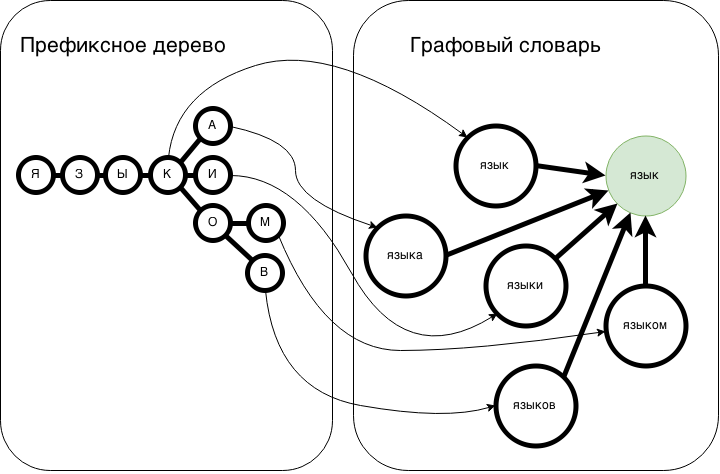
\includegraphics[scale=0.6]{img/prefixtree.png}
	\caption{Пример фрагмента префиксного дерева}
\end{figure}

\subsubsection{Редакционное расстояние}
Редакционное расстояние между двумя строками в компьютерной лингвистике является метрикой, равной количеству редакционных правок, необходимых для преобразования первой строки во вторую. Очевидно, редакционное расстояние между двумя одинаковыми строками равно \(0\):
\begin{align}
	dist(S_1, S_2) = 0 \Leftrightarrow S_1 = S_2\text{.}
\end{align}
Также следует отметить свойство коммутативности редакционного расстояния:
\begin{align}
	dist(S_1, S_2) = dist(S_2, S_1)\text{.}
\end{align}
Вычисление редакционного расстояния может быть осуществлено с помощью алгоритмов динамического программирования \cite{dasgupta}. Идея динамического программирования заключается в формировании множества подзадач, в которое входит и исходная задача, и решении задач из этого множества в ``правильном'' порядке. 

В данной работе используется редакционное расстояние Левенштейна \cite{manning}. В рамках редакционного расстояния Левенштейна определены следующие виды редакционных правок:
\begin{itemize}
	\item
	вставка одного символа;
	\item
	удаление одного символа;
	\item
	замена одного символа.
\end{itemize}
Рекуррентная формула вычисления редакционного расстояния Левенштейна выглядит следующим образом:
\begin{align} 
	M &= |S_1|, N = |S_2|, \\
	dist(S_1, S_2) &= D(M, N) \\
	D(i, j) &= 
	\begin{cases}
		0&,\text{ если } i = 0, j = 0 \\
		j&,\text{ если } i = 0, j > 0 \\
		i&,\text{ если } j = 0, i > 0 \\
		min(\substack{
			D(i, j - 1) + 1, \\
			D(i - 1, j) + 1, \\
			D(i - 1, j - 1) + cmp(S_1[i], S_2[j])
		})&,\text{ если } i > 0, j > 0 \\  
	\end{cases}
\end{align}
В приведенной рекуррентной формуле цена удаления или вставки символа равна \(1\). \(cmp(c_1, c_2)\) - функция, принимающая два символа как аргументы и возвращающая цену замены символа \(c_1\) на \(c_2\). Очевидно, что \( cmp(c_1, c_2) = 0 \Leftrightarrow c_1 = c_2\). Если \(c_1 \neq c_2\), то \( cmp(c_1, c_2) > 0 \) и, в таком случае возможен учет, например, физического расстояния между клавишами, соответствующими данным символам в какой-либо раскладке. Следует отметить, что ``промах'' по клавишам является очень частой ошибкой при наборе текста. Особенно часто такие дефекты встречаются в текстах, набираемых в спешке. Такого вида тексты широко представлены на просторах сети Интернет и могут представлять интерес для различного рода исследований, для поддержи которых и предназначены системы автоматической обработки текста.

Рассмотрим способ применения динамического программирования для вычисления редакционного расстояния Левенштейна по вышеприведенной формуле. \(D(i, j)\) - расстояние между префиксами строк. Если \(|S_1| = M\), а \(|S_2| = N\), то наша конечная цель - вычисление \(D(M, N)\). Чтобы достичь этой цели, нужно выразить \(D(M, N)\) через более простые подзадачи \(D(M', N')\), где \(M' \leq M, N' \leq N\). Таким образом, решение подзадач можно представить как заполнение матрицы размера \(M\) на \(N\). Причем на порядок заполнения матрицы накладывается только одно ограничение: \(D(i - 1, j - 1)\), \(D(i - 1, j)\), \(D(i, j - 1)\) должны быть вычислены раньше \(D(i, j)\).
\begin{figure}[H]
	\centering
	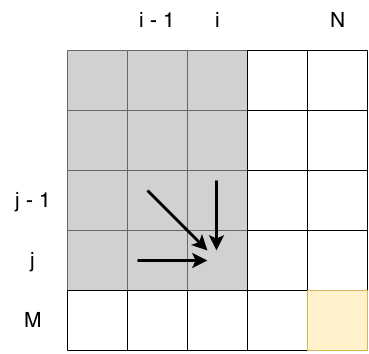
\includegraphics[scale=0.5]{img/levenstein.png}
	\caption{Иллюстрация вычисления расстояния Левенштейна методом динамического программирования}
\end{figure}
\begin{lstlisting}[caption={Пример реализации вычисления расстояния Левенштейна}, language=Java]
public static int dist(String s1, String s2) {
    int[][] d = new int[s1.length() + 1][s2.length() + 1];
    for(int i = 0; i <= s1.length(); i++) {
        for(int j = 0; j <= s2.length(); j++) {
            if(i == 0 && j == 0) {
                d[i][j] = 0;
            } else if (i == 0 && j > 0) {
                d[i][j] = j;
            } else if (j == 0 && i > 0) {
                d[i][j] = i;
            } else {
                d[i][j] = min(
                				d[i][j - 1] + 1, 
                				d[i - 1][j] + 1,
                        		d[i - 1][j - 1] + cmp(
                        								s1.charAt(i - 1), 
                        								s2.charAt(j - 1)
                        							 )
                        	 );
            }
        }
    }
    return d[s1.length()][s2.length()];
}
\end{lstlisting}

\subsubsection{Алгоритм нечеткого поиска}
Алгоритм нечеткого поиска, используемый в данной работе, построен таким образом, чтобы выполнять поиск по построенному префиксному дереву поиска. В рамках работы алгоритма определяется список путей прохождения по дереву, которые представляют собой потенциальные нечеткие (аппроксимационные) совпадения с искомой словоформой. Каждый путь ассоциирован с редакционным расстоянием между результирующим префиксом и соответствующим ему префиксом искомой словоформы. На каждом шаге:
\begin{itemize}
	\item
	префикс словоформы увеличивается на один символ;
	\item
	список путей дополняется путями, полученными добавлением дочерних узлов дерева поиска к имеющимся путям;
	\item
	для каждого пути в списке пересчитывается редакционное расстояние;
	\item
	пути, редакционное расстояние для которых превышает некоторое пороговое значение, отбрасываются.
\end{itemize}
\begin{figure}[H]
	\centering
	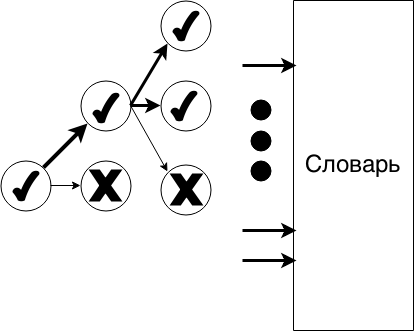
\includegraphics[scale=0.6]{img/treesearch.png}
	\caption{Иллюстрация алгоритма нечеткого поиска}
\end{figure}
В результате нечеткого поиска могут выделяться части искомой словоформы как отдельные токены. Именно на этом этапе и появляются различные варианты разбиения. Следует отметить, с каждым путем из списка текущих путей, помимо вычисленного редакционного расстояния, также ассоциирована матрица вычисления расстояния Левенштейна. Это сделано из тех соображений, что при добавлении одного символа к сравниваемым строкам или к одной из них матрица вычисления расстояния дополняется пустым столбцом и/или одной пустой строкой. Полученная матрица удовлетворяет указанному ранее условию: \(D(i - 1, j - 1)\), \(D(i - 1, j)\), \(D(i, j - 1)\) должны быть вычислены раньше \(D(i, j)\). Исходя из этого, для нового пути нет необходимости пересчитывать всю матрицу: достаточно заполнить только новый столбец и/или строку.
\begin{figure}[H]
	\centering
	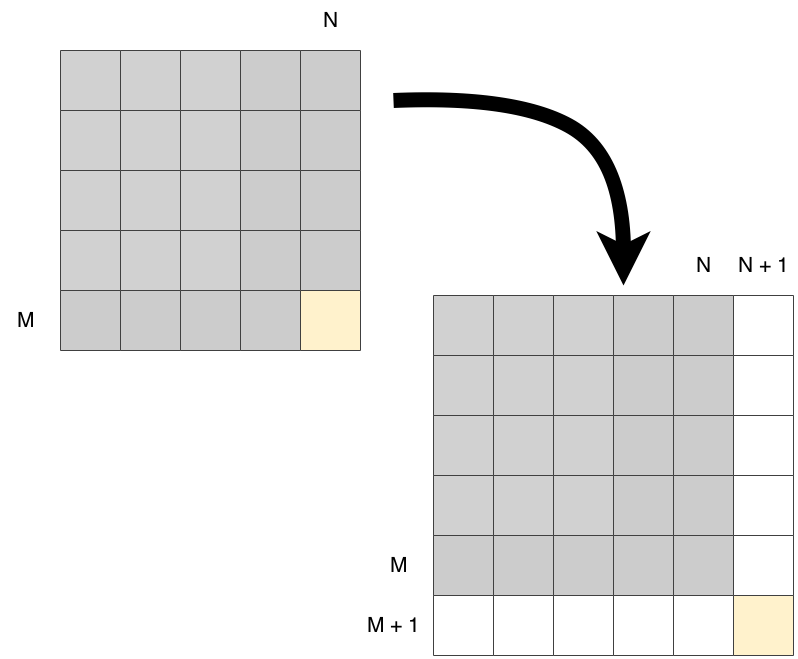
\includegraphics[scale=0.5]{img/matrixrecompute.png}
	\caption{Пересчет матрицы вычисления редакционного расстояния}
\end{figure}

\subsubsection{Модель n-грамм}
Модель n-грамм является одной из языковых моделей. Данная модель представляет собой вероятностную модель. Ключевым понятием данной модели является n-грамма. Модель позволяет вычислить вероятность встретить какую-либо последовательность (предложение) или найти вероятность встретить какое-либо слово в конце последовательности слов:
\begin{itemize}
	\item
	предложение
	\begin{align}
		W = w_1w_2w_3w_4w_5...w_n;
	\end{align}
	\item
	вероятность встретить такое предложение
	\begin{align}
		P(W) = P(w_1w_2w_3w_4w_5...w_n);
	\end{align}
	\item
	вероятность встретить слово в конце предложения
	\begin{align}
		P(w_n|w_1w_2w_3w_4w_5...w_{n-1}).
	\end{align}
\end{itemize}
Естественным образом можно рассуждать, основываясь на теореме об умножении вероятностей \cite{gmurman}:
\begin{align}
	P(AB) = P(A) \cdot P_A(B).
\end{align}
В общем случае:
\begin{align}
	P(x_1x_2x_3...x_n) = P(x_1)P(x_2|x_1)P(x_3|x_1x_2)...P(x_n|x_1...x_{n-1}).
\end{align}
Применяя данную теорему к вероятности встречи предложения, получим:
\begin{align}
	P(w_1w_2w_3...w_n) = \prod_{i}P(w_i|w_1w_2w_3...w_{i-1})
\end{align}
Применить данную формулу для расчета вероятностей встречи того или иного предложения не представляется возможным ввиду отсутствия практической возможности получения данных в необходимом объеме. Количество различных последовательностей слов слишком велико, чтобы иметь возможность рассчитать вероятность встречи той или иной последовательности произвольной длины на основе частоты ее встречаемости. Ввиду вышесказанного делается допущение, что появление слов в предложении обладает Марковским свойством:
\begin{align}
	P(w_i|w_1w_2w_3...w_{i-1}) \approx P(w_i|w_{i-k}...w_{i-1}).
\end{align}
Тогда
\begin{align}
	P(w_1w_2w_3...w_n) = \prod_{i}P(w_i|w_{i-k}...w_{i-1}).
\end{align}
\(k\) определяет максимальное количество слов в последовательности, в которой появление последнего слова зависит от первого слова. В соответствии с \(k\) различают, например, следующие частные случаи:
\begin{itemize}
	\item
	модель униграмм
	\begin{align}
		&k = 0, \nonumber \\
		&P(w_i|w_1w_2w_3...w_{i-1}) \approx P(w_i), \\
		&P(w_1w_2w_3...w_n) = \prod_{i}P(w_i); 
	\end{align}
	\item
	модель биграмм
	\begin{align}
		&k = 1, \nonumber \\
		&P(w_i|w_1w_2w_3...w_{i-1}) \approx P(w_i|w_{i-1}), \\
		&P(w_1w_2w_3...w_n) = \prod_{i}P(w_i|w_{i-1});
	\end{align}
	\item
	модель триграмм
	\begin{align}
		&k = 2, \nonumber \\
		&P(w_i|w_1w_2w_3...w_{i-1}) \approx P(w_i|w_{i-1}w_{i-2}), \\
		&P(w_1w_2w_3...w_n) = \prod_{i}P(w_i|w_{i-1}w_{i-2}).
	\end{align}
\end{itemize}
В данной работе используется модель биграмм ввиду того, что частотные списки биграмм шире представлены.
\subsubsection{Ранжирование результатов}
Ранжирование результатов осуществляется в соответствии с мультипликативным критерием, учитывающим суммарное редакционное расстояние и вероятность, вычисленную в соответствии с моделью n-грамм. Пусть имеется результат аннотирования \(W = w_1w_2w_3...w_n\). Суммарное редакционное расстояние можно вычислить так:
\begin{align*}
	\displaystyle\sum_{j} dist(w_j,w_{dict_j}) .
\end{align*}
Максимальное редакционное расстояние расчитывается исходя из свойства
\begin{align}
	dist(S_1, S_2) \leq max(|S_1|, |S_2|).
\end{align}
Тогда максимальное суммарное редакционное расстояние можно вычислить следующим образом:
\begin{align*}
	\displaystyle\sum_{j} max(|w_j|,|w_{dict_j}|) .
\end{align*}
При такой формулировке степень несовпадения можно определить, как
\begin{align*}
	\frac{\displaystyle\sum_{j} dist(w_j,w_{dict_j}) }{\displaystyle\sum_{j} max(|w_j|,|w_{dict_j}|) }
\end{align*}
Тогда степень совпадения можно определить так:
\begin{align*}
	1 - \frac{\displaystyle\sum_{j} dist(w_j,w_{dict_j}) }{\displaystyle\sum_{j} max(|w_j|,|w_{dict_j}|) }
\end{align*}
Итоговый критерий определяется следующим образом:
\begin{align}
	k(W) = \left(1 - \frac{\displaystyle\sum_{j} dist(w_j,w_{dict_j}) }{\displaystyle\sum_{j} max(|w_j|,|w_{dict_j}|) }\right) \cdot \prod_{j}P(w_j|w_{j-1}).
\end{align}
\(W_1\) считается лучше \(W_2\), если \(k(W_1) > k(W_2)\).

	\FloatBarrier
	\clearpage

	\section{Практическая реализация}
	На основе предложенного подхода к предсинтаксическому аннотированию текста на естественном языке был разработан программный модуль, выполняющий данную задачу. Разработанный программный модуль интегрирован в систему семантического анализа. Исходные коды данного программного модуля написаны на языке Java. На первой фазе разработанного подхода используется скрытая марковская модель. Скрытая марковская модель реализована на основе исходных кодов библиотеки JHMM, распространяемых под лицензией New BSD License \cite{nbsd}. Возможности данной библиотеки были расширены: реализован алгоритм обучения скрытой марковской модели с учителем, описанный в предыдущем разделе. Для этого был применен паттерн декоратор \cite{gof}.
\begin{figure}[H]
	\centering
	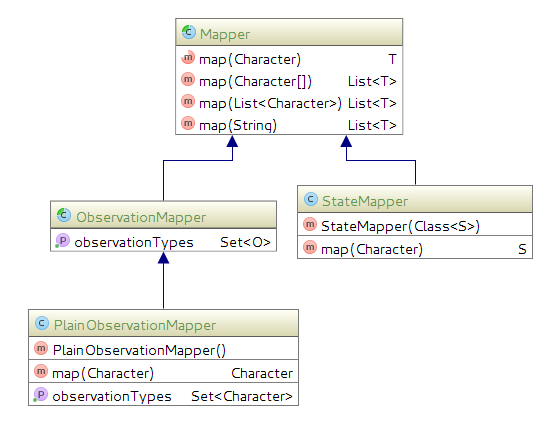
\includegraphics[scale=0.7]{img/uml_mappers.png}
	\caption{Иерархия классов, предназначенных для отображения множеств наблюдений и состояний}
\end{figure}
Для достижения возможности введения дополнительных скрытых состояний модели и определения различных множеств наблюдений был введен дополнительный уровень абстракции. На данном уровне абстракции производится отображение множества наблюдений, представленного множеством символов Юникода, в другое множество наблюдений, определяемое конкретным экспериментом. 

Обучающее множество было подготовлено на основе размеченного лингвистического корпуса, составляемого в рамках проекта ``Национальный корпус русского языка'' \cite{natcorp_1, natcorp_2}. Корпус доступен для некоммерческого использования. В рамках предложенного подхода определено три скрытых состояния: внутри токена, вне токена, граница токена. Обучающее множество представляет собой множество размеченных предложений.
\begin{lstlisting}[caption={Фрагмент обучающего множества}]
 Мне жаль что тебя не застал летний ливень 
 bwb bwwb bwb bwwb bb bwwwwb bwwwwb bwwwwb
 В июльскую ночь на Балтийском заливе 
 b bwwwwwwb bwwb bb bwwwwwwwwb bwwwwb
 Не видела ты волшебства этих линий.
 bb bwwwwb bb bwwwwwwwwb bwwb bwwwb
 Волна, до которой приятно коснуться руками 
 bwwwb  bb bwwwwwb bwwwwwb bwwwwwwwb bwwwwb
 Песок, на котором рассыпаны камни 
 bwwwb  bb bwwwwwb bwwwwwwwb bwwwb
 Пейзаж, не меняющийся здесь веками.
 bwwwwb  bb bwwwwwwwwb bwwwb bwwwwb
 Мне жаль что мы снова не сядем на поезд 
 bwb bwwb bwb bb bwwwb bb bwwwb bb bwwwb
 Который пройдёт часовой этот пояс 
 bwwwwwb bwwwwwb bwwwwwb bwwb bwwb
 По стрелке которую тянет на полюс.
 bb bwwwwwb bwwwwwb bwwwb bb bwwwb
\end{lstlisting}
Каждое предложение представлено последовательностью символов алфавита естественного языка. Для каждого символа предложения поставлено в соответствие скрытое состояние. Состоянию ``граница токена'' соответствует символ ``b'', состоянию ``внутри токена'' соответствует символ ``w'', a состоянию вне токена соответствует символ `` ''. Подготовка обучающего множества заключается в преобразовании множества размеченных текстов, входящих в состав лингвистического корпуса, в множество размеченных предложений. 

В работе проведено тестирование, целью которого было составление представления об объеме обучающего множества, необходимом для достижения малой доли ошибок разметки текста. Полученное на основе лингвистического корпуса обучающее множество было разделено на две части. Первая часть использовалась алгоритмом обучения с учителем для обучения скрытой марковской модели, а вторая - для тестирования. При этом были выбраны предложения, размер которых составлял 5 - 10 слов. Количество предложений в части обучающего множества, на которой производилось обучение, изменялось от 0 до 5000 с шагом в 10 предложений. Доля ошибок рассчитывалась как отношение количества предложений, в которых была допущена хоть одна ошибка разметки, к количеству предложений в тестовом множестве.
\begin{figure}[H]
	\centering
	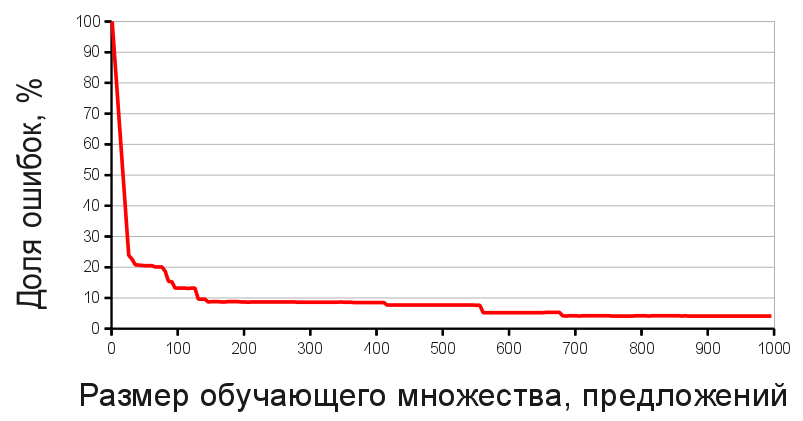
\includegraphics[scale=0.5]{img/test_chart.png}
	\caption{Доля ошибок разметки в зависимости от объема обучающего множества}
\end{figure}
В ходе тестирования было выявлено, что при достижении объема обучающего множества 690 предложений, дальнейшее увеличение объема обучающего множества не приводит к значительному изменению доли ошибок разметки.

Для реализации графового словаря была выбрана графовая база данных OrientDB \cite{web.orient}. Выбор обусловлен наличием как объектного, так и реляционного интерфейса доступа к данным, а также наличием бинарного интерфейса поверх протокола TCP, что делает возможным обращение к данной базе данных из нативного кода без использования сторонних библиотек. Последняя возможность особенно важна ввиду того, что часть модулей системы семантического анализа написаны на языке C++.

Разработанный программный модуль предсинтаксического аннотирования текста разработан на языке Java. Сборка производится посредством системы сборки Maven \cite{maven}. Модуль доступен в виде библиотеки JAR.

Запуск предсинтаксического аннотирования осуществляется посредством вызова метода tokenize класса, реализующего интерфейс Tokenizer. Для получения экземпляра используется паттерн фабрика \cite{gof}.
\begin{lstlisting}[caption={Интерфейс модуля предсинтаксического аннотирования}]
public interface Tokenizer {

    /**
     * Выполнение предсинтаксического аннотирования текста
     *
     * @param   in  входной поток символов
     * @return      ранжированный список результатов
     */
    List<TokenizationResult> tokenize(InputStream in);

}
\end{lstlisting}
Метод tokenize возвращает ранжированный список результатов предсинтаксического аннотирования. Результат аннотирования реализует интерфейс TokenizationResult, позволяющий получить список найденных токенов и значение критерия ранжирования, соответствующее данному результату.
\begin{lstlisting}[caption={Интерфейс результата аннотирования}]
public interface TokenizationResult {

    /**
     * Получение значения критерия ранжирования 
     * для данного результата
     */
    double getK();

    /**
     * Получение списка токенов
     */
    List<Token> getTokens();

}
\end{lstlisting}
Токен имеет интерфейс, позволяющий получить исходную последовательность символов, соответствующую найденному токену, и последовательность символов с внесенными корректировками. Также имеется возможность получить список установленных атрибутов и ссылку на узел графового словаря, если найденный токен является словоформой.
\begin{lstlisting}[caption={Интерфейс токена}]
public interface Token {

    /**
     * Исходная последовательность символов,
     * соответствующая данному токену
     */
    char[] getSeq();

    /**
     * Последовательность символов с применением корректировок,
     * соответствующая данному токену
     */
    char[] getModifiedSeq();

    /**
     * Ссылка на узел графового словаря
     */
    Long getDictNodeId();

    /**
     * Список установленных атрибутов
     */
    List<Attribute> getAttributes();

}
\end{lstlisting}
	\FloatBarrier
	\clearpage

	\section{Результат}
	В результате исследования был найден подход к предсинтаксическому аннотированию текста, соответствующий поставленным требованиям:
\begin{enumerate}
	\item 
	возможность разметки текста, содержащего дефекты;
	\item
	возможнотсь одновременной работы с несколькими языками;
	\item
	представление результата в виде ссылок на записи морфологического словаря.
\end{enumerate}

Предложен двухэтапный алгоритм, построенный на основе использования скрытой марковской модели и нечеткого поиска по морфологическому словарю.

Разработан программный модуль, выполняющий предсинтаксическое аннотирование текста на естественном языке. В ходе тестирования определены требования к объему обучающего множества, используемого для обучения скрытой макрковской модели.
	\FloatBarrier
	\clearpage

	\section{Библиографический список}
	\bibliography{bibliography}
	\clearpage

\end{document}
